\documentclass[11pt]{article}
\pdfinfoomitdate=1
\pdftrailerid{}
\pdfsuppressptexinfo=15
\usepackage[T1]{fontenc}
\usepackage{lmodern,microtype,amsmath,amssymb,amsthm,mathtools,booktabs}
\usepackage[margin=1.05in]{geometry}
\usepackage{tikz}
\usetikzlibrary{arrows.meta,positioning}
\usepackage[colorlinks=true,linkcolor=blue,citecolor=blue,urlcolor=blue]{hyperref}
\hypersetup{pdftitle={A strict four-row permanent inequality and permutation moments},pdfauthor={OpenAI}}
\newtheorem{theorem}{Theorem}[section]
\newtheorem{lemma}[theorem]{Lemma}
\newtheorem{proposition}[theorem]{Proposition}
\newtheorem{corollary}[theorem]{Corollary}
\theoremstyle{remark}\newtheorem{remark}[theorem]{Remark}
\DeclareMathOperator{\Tr}{Tr}
\DeclareMathOperator{\tr}{tr}
\DeclareMathOperator{\TV}{TV}
\DeclareMathOperator{\op}{op}
\DeclareMathOperator{\Res}{Res}
\DeclareMathOperator{\Ind}{Ind}
\newcommand{\E}{\mathbb E}
\newcommand{\Pp}{\mathbb P}
\newcommand{\one}{\mathbf1}
\newcommand{\sgn}{\mathrm{sgn}}
\newcommand{\HS}{\mathrm{HS}}
\newcommand{\norm}[1]{\left\lVert#1\right\rVert}
\title{A strict four-row permanent inequality and permutation moments}
\author{OpenAI}
\date{September 26, 2026}
\begin{document}
\maketitle
\begin{abstract}
We prove a permanent inequality with exponent strictly below two for laws on $S_4$ sufficiently close to uniform and with exactly uniform coordinate marginals. Applied to a four-row recursion, it shows that an absolute number of coordinate sweeps brings the full permutation of the Thorp shuffle on $N=2^d$ cards to total-variation distance tending to zero from uniform as $N\to\infty$. Thus the mixing time has the optimal order $O(\log N)$ in physical shuffles.
\end{abstract}
\section{Introduction}
A product of independent random switches can make each card uniform while leaving substantial dependence between cards. The Thorp shuffle illustrates this distinction particularly well. On $N=2^d$ positions, with $d\ge1$, one coordinate sweep visits the binary-coordinate directions in the fixed order $1,\ldots,d$. In each direction it independently swaps the two cards on every edge with probability $1/2$, leaving them in place otherwise. Every individual card is uniform after this sweep. The question is how many sweeps randomize the entire permutation.

We study that question through a four-row decomposition. Removing two coordinate directions leaves four smaller independent sweeps, one in each row of a $4$-by-$N/4$ array. The last two directions act within its columns. Each smaller sweep contracts according to the representations of its own row group, but restricting a representation of $S_N$ to the four row groups creates multiplicities. Those multiplicities accumulate as the decomposition is repeated. The main point is an inequality that makes their total cost strictly smaller than the available representation dimension.

For a function $f:\{1,2,3,4\}\to[0,\infty)$, write
\[
 \|f\|_p=\left(\frac14\sum_{j=1}^4 f(j)^p\right)^{1/p}.
\]
If $u$ denotes uniform measure on $S_4$, then
$\E_u\prod_i f_i(\pi(i))$ is the permanent of the matrix $(f_i(j))$ divided by $4!$. Carlen, Lieb and Loss proved that it is at most $\prod_i\|f_i\|_2$ and characterized equality \cite[Theorem~1.1]{cll2006}. For nonzero nonnegative functions on four points, equality requires that every function be constant. We will use both the bound and this equality statement.

\begin{samepage}
\begin{theorem}[A robust four-row inequality]
There are absolute constants $p_0\in(4/3,2)$ and $\varepsilon>0$ with the following property.\label{thm:permanent} Let $\nu$ be a probability measure on $S_4$ such that
\[
 \|\nu-u\|_{\TV}<\varepsilon,
 \qquad
 \nu\{\pi:\pi(i)=j\}=\frac14\quad(1\le i,j\le4).
\]
Then every four nonnegative functions on $\{1,2,3,4\}$ satisfy
\begin{equation}\label{eq:permanent}
 \E_\nu\prod_{i=1}^4f_i(\pi(i))\le\prod_{i=1}^4\|f_i\|_{p_0}.
\end{equation}
\end{theorem}
\end{samepage}

Here total variation is one half the sum of the absolute differences of the probability masses. The marginal assumption in the theorem is exact. Indeed, setting three functions equal to one in \eqref{eq:permanent}, and varying the fourth around the constant one, forces its coordinate marginal to be uniform. Thus this hypothesis describes a structural feature of the inequality, as well as the cancellation used in its proof.

Permanents with row or column $\ell^p$ constraints have a broader history. Carlen--Lieb--Loss discuss the below-two problem and Caputo's conjecture, and Samorodnitsky obtained further bounds in that range \cite{cll2006,Samorodnitsky2008}. Bristiel and Caputo subsequently proved the sharp permanent bound for every $p\ge1$ \cite[Corollary~1.14]{BristielCaputo2024}. In the present normalization, their result gives
\[
 \E_u\prod_i f_i(\pi(i))\le\prod_i\|f_i\|_p
 \quad\text{for every }p\ge p_c:=\frac{4\log4}{\log24}.
\]
The identity matrix shows that this uniform-law threshold is necessary.

The assertion needed here is stability under small perturbations of the permutation law that preserve every coordinate marginal. We prove this nonoptimal robust form directly from the exponent-two theorem: a strict quadratic gap treats functions near constants, while the equality classification and compactness treat all remaining functions. The local calculation explains the endpoint $4/3$ in Theorem~\ref{thm:permanent}; the final exponent is chosen closer to two and is not optimized. Thus a below-two bound for the uniform law is not itself the new ingredient in the recursion.

To state the application, let $\rho_\lambda$ be the irreducible unitary representation of $S_N$ indexed by a partition $\lambda\vdash N$, and write $D_\lambda$ for its dimension and $\lambda'$ for the conjugate partition. If $\mu_N$ is the law of one sweep, put
\[
 T_N(\lambda)=\sum_{g\in S_N}\mu_N(g)\rho_\lambda(g),
 \qquad B_N(\lambda)=T_N(\lambda)T_N(\lambda)^*.
\]
Traces are ordinary, unnormalized matrix traces. Unmarked logarithms are natural.

\begin{theorem}[A fixed moment with a degree saving]\label{thm:moment}
There exist an even integer $r\ge2$ and $\eta>0$, independent of $N$, such that for every dyadic $N$ and every $\lambda\vdash N$,
\begin{equation}\label{eq:moment}
 D_\lambda\Tr B_N(\lambda)^r\le D_\lambda^{1-\eta}.
\end{equation}
Consequently there is an absolute integer $q$ for which the total-variation distance of $q$ independent forward sweeps from uniform tends to zero as $N\to\infty$, uniformly over the starting deck.
\end{theorem}

A physical Thorp shuffle consists of independent fair switches on the pairs differing in one binary coordinate, followed by cyclic rotation of the coordinates. Tracking those deterministic rotations makes $d$ physical shuffles exactly one sweep. Theorem~\ref{thm:moment} therefore gives an $O(d)$ upper bound. The opposite order follows from the elementary support estimate
\begin{equation}\label{eq:support-intro}
 \|\mu_t-U_{S_N}\|_{\TV}\ge1-\frac{2^{tN/2}}{N!},
\end{equation}
where $\mu_t$ is the law after $t$ physical shuffles: there are only $2^{tN/2}$ coin strings. In particular, distance at most $1/4$ requires
$t\ge\lceil(2/N)\log_2(3N!/4)\rceil=2d-O(1)$.

The shuffle originates in Thorp's study of nonrandom shuffling and Faro \cite{Thorp1973}. For $N=2^d$, Morris obtained an $O(d^{44})$ upper bound \cite{Morris2008}, and Montenegro and Tetali improved it to $O(d^{29})$ \cite[Theorems~6.14--6.15]{MontenegroTetali2006}. Morris subsequently proved $O((\log N)^4)$ for every even deck size \cite{Morris2009} and $O(d^3)$ for dyadic decks \cite{Morris2013}. The present proof reaches logarithmic order through a four-row moment recursion.

The proof has three stages. Section~\ref{sec:permanent} proves the robust inequality and tensors it over columns. In Section~\ref{sec:recursion}, a positive trace comparison reduces the sweep moment to four smaller moments, multiplied by powers of squared restriction multiplicities. The power is
$\theta=1-1/p_0<1/2$: this strict improvement over one half is the feature the dimension comparison needs. Section~\ref{sec:multiplicities} bounds the multiplicities by removing the first few rows and columns of a Young diagram. Horizontal and vertical Pieri rules control the removed strips. For every fixed width $h$, the total number of boxes outside the first $h$ rows and columns of the four child diagrams is at most the corresponding number in the parent. We deduce this inequality from positive hook-Schur specialization, originating with Berele--Regev \cite{BereleRegev1987}; the formulas and tableau conventions used here are recorded in \cite{orellana-zabrocki2000,mason-niese2016}.

Finally, Section~\ref{sec:sparse} stops the recursion for diagrams close to a row or column. Section~\ref{sec:tree} sums the costs at every other scale, including the immediate children at which recursion has stopped, and compares the result with the hook-length formula. The strict inequality $\theta<1/2$ is exactly the margin that absorbs these costs. Section~\ref{sec:amplification} converts the resulting moment to mixing. This last step follows the finite-group Fourier approach of Diaconis--Shahshahani \cite{DiaconisShahshahani1981}, with matrix norms retained because a sweep is generally nonnormal.

The argument uses ordinary complex representation theory of symmetric groups: branching, induction and restriction, the Littlewood--Richardson and Pieri rules, and the hook-length formula \cite{James1978,Sagan2001,Stanley1999}. We give the additional multiplicity and dimension estimates in full. The positive trace comparison is the Araki--Lieb--Thirring inequality \cite{araki1990}. No shuffle moment or mixing theorem from another source is an input here.

\section{The strict permanent inequality}\label{sec:permanent}
We first prove Theorem~\ref{thm:permanent}. The two parts of the proof address different possible failures of a uniform improvement: functions close to the equality cases, and functions bounded away from them.

\begin{proof}[Proof of Theorem~\ref{thm:permanent}]
A zero function makes the assertion immediate. By homogeneity, normalize each nonzero function to have $\|f_i\|_2=1$. The resulting space of quadruples is compact. The exponent-two Carlen--Lieb--Loss inequality is strict everywhere on this space except at the single quadruple $f_i\equiv1$. Its normalization follows directly from
\[
 \operatorname{perm}(f_i(j))\le\frac{4!}{4^2}
       \prod_i\left(\sum_j f_i(j)^2\right)^{1/2}.
\]
The equality classification for nonzero nonnegative columns gives exactly the stated exceptional quadruple \cite[Theorem~1.1 and equation~(1.4)]{cll2006}.

All scalar expectations and inner products on four points use uniform measure:
$\E_jh(j)=\tfrac14\sum_jh(j)$ and $\langle g,h\rangle=\tfrac14\sum_jg(j)h(j)$.
Fix $p_*\in(4/3,2)$. Near that quadruple, the means are positive, so renormalize by the means and write $f_i=1+g_i$, with $\E_jg_i(j)=0$. Let
\[
 V=\sum_i\|g_i\|_2^2,\qquad b=\max_i\|g_i\|_\infty.
\]
For $i\ne j$, uniform sampling without replacement gives
\[
 \E_u g_i(\pi(i))g_j(\pi(j))
 =-\frac13\langle g_i,g_j\rangle.
\]
Consequently the total quadratic term is
\begin{equation}\label{eq:quadratic}
 \sum_{i<j}\E_u g_i(\pi(i))g_j(\pi(j))
 =\frac16\left(V-\Big\|\sum_i g_i\Big\|_2^2\right)
 \le\frac V6.
\end{equation}

For a law $\nu$ at total-variation distance at most $\varepsilon$ from $u$, the change in each quadratic expectation is at most
$2\varepsilon\|g_i\|_\infty\|g_j\|_\infty$. On four points, $\|g_i\|_\infty\le2\|g_i\|_2$, so the total change is at most an absolute constant times $\varepsilon V$. All linear terms are zero under $\nu$, because every coordinate marginal is uniform. Each cubic or quartic term is at most an absolute constant times $bV$ when $b\le1/2$. Indeed, bound all but two factors by $b$ and apply Cauchy--Schwarz to the remaining factors; their squared expectations use only the uniform marginals. Thus
\begin{equation}\label{eq:lhs-local}
 \E_\nu\prod_i(1+g_i(\pi(i)))
 \le1+\left(\frac16+C\varepsilon+Cb\right)V.
\end{equation}

Taylor's formula on $[1/2,3/2]$, uniformly for $p\in[p_*,2]$, gives
\[
 \E_j(1+g_i(j))^p
 =1+\frac{p(p-1)}2\|g_i\|_2^2
          +O\bigl(b\|g_i\|_2^2\bigr).
\]
Taking $p$th roots and multiplying the four factors gives
\begin{equation}\label{eq:rhs-local}
 \prod_i\|1+g_i\|_p
 =1+\frac{p-1}2 V+O(bV).
\end{equation}
All constants are uniform on the fixed interval of exponents. Since
$(p_*-1)/2>1/6$, first choose $b_*>0$ and $\varepsilon_*>0$ small enough that the error terms in \eqref{eq:lhs-local} and \eqref{eq:rhs-local} fit inside this strict gap. The desired inequality then holds for every $p\in[p_*,2]$ whenever $b<b_*$ and $\|\nu-u\|_{\TV}\le\varepsilon_*$, with exact uniform marginals.

Return to the $L^2$-normalized compact space. The condition just obtained contains a fixed open neighborhood $\mathcal U$ of its constant quadruple. On the compact complement of $\mathcal U$, the exponent-two inequality has a positive minimum gap. Both sides are continuous in the functions; they are also continuous in the exponent and in the probability masses of $\nu$. Choose $p_0\in[p_*,2)$ sufficiently close to two, then $0<\varepsilon\le\varepsilon_*$ sufficiently small, so that this gap remains positive on the complement. The local argument applies on $\mathcal U$ with these same constants. These two regions cover all normalized quadruples, proving the theorem.
\end{proof}

The exact marginal assumption can also be read off without Taylor estimates of second order. If $a(j)=\nu\{\pi(i)=j\}-1/4$ is nonzero, choose $g=a$ and set $f_i=1+t g$, with the other functions one. The derivative at $t=0$ of the left side minus the right side of \eqref{eq:permanent} is $\sum_j a(j)^2>0$. Small positive $t$ contradicts the inequality.

\begin{lemma}[Tensorization]\label{lem:tensorization}
Let $\pi_1,\ldots,\pi_b$ be independent random permutations, each with a law satisfying Theorem~\ref{thm:permanent} for the same $p_0$. If $F_i$ is a nonnegative function on $\{1,2,3,4\}^b$, then
\[
 \E\prod_{i=1}^4 F_i(\pi_1(i),\ldots,\pi_b(i))
 \le\prod_{i=1}^4
 \left(4^{-b}\sum_{x\in\{1,2,3,4\}^b}F_i(x)^{p_0}\right)^{1/p_0}.
\]
\end{lemma}
\begin{proof}
Induct on $b$. Fix the first $b-1$ coordinates and apply Theorem~\ref{thm:permanent} to the last coordinate. The four resulting functions on $b-1$ coordinates are
\[
 G_i(x)=\left(\frac14\sum_{j=1}^4 F_i(x,j)^{p_0}\right)^{1/p_0}.
\]
The induction hypothesis applies to their product, and its $p_0$th-power sums are precisely the full product-measure sums in the assertion.
\end{proof}

For later use, let $U$ be a positive semidefinite stochastic matrix of order $s$. Its entries are nonnegative and its eigenvalues lie in $[0,1]$. H\"older's inequality, applied entry by entry with powers $2-p_0$ and $p_0-1$, gives
\begin{equation}\label{eq:interpolation}
 \sum_{x,y}U(x,y)^{p_0}
 \le\left(\sum_{x,y}U(x,y)\right)^{2-p_0}
       \left(\sum_{x,y}U(x,y)^2\right)^{p_0-1}
 \le s^{2-p_0}(\Tr U)^{p_0-1}.
\end{equation}
The final inequality uses $\Tr U^2\le\Tr U$. Taking the $p_0$th root with the uniform counting normalization gives
\[
 \left(s^{-2}\sum_{x,y}U(x,y)^{p_0}\right)^{1/p_0}
 \le s^{-1}(\Tr U)^{1-1/p_0}.
\]
Section~\ref{sec:recursion} applies this estimate to four color-string transition matrices. Each contributes a factor $s^{-1}$ and a trace power $\theta=1-1/p_0$. The strict inequality $\theta<1/2$ will remain fixed throughout the proof.

\section{From columns to a four-row moment recursion}\label{sec:recursion}
Our objective is to express a moment on $N$ cards in terms of moments on $N/4$ cards. We first fix the operator conventions, then isolate the cost of the interaction between the four rows.

Positions are binary vectors. A permutation sends input positions to output positions, and $gh$ applies $h$ first. In each coordinate direction, the average of all optional edge swaps is an orthogonal projection $\Pi_i$. With chronological order $1,\ldots,d$,
\[
 T_N=\Pi_d\cdots\Pi_1,\qquad B_N=T_NT_N^*.
\]
To check physical time, let $R(x_1,\ldots,x_d)=(x_2,\ldots,x_d,x_1)$ and let $S_t$ be the switches in the first coordinate. A physical step is $RS_t$. If $Y_t$ is the accumulated permutation, then $X_t=R^{-t}Y_t$ satisfies
\[
 X_{t+1}=(R^{-t}S_{t+1}R^t)X_t.
\]
The conjugated directions visit all coordinates in a fixed cyclic order, and $R^d=I$. Relabeling that order as $1,\ldots,d$ gives exactly $T_N$ after $d$ steps.

These are group-algebra elements as well as operators in any representation. The Fourier transform convention is $\widehat\mu(\lambda)=\sum_g\mu(g)\rho_\lambda(g)$; convolution multiplies these matrices in the same order. For a matrix $A$, the unnormalized Schatten norm is $\|A\|_p^p=\Tr|A|^p$.

\begin{lemma}[Annihilation and the finite-size gap]\label{lem:gap}
Every sweep kills the sign representation and every shape with more than $N/2$ rows. For fixed dyadic $N\ge2$, its operator norm on each nontrivial irreducible representation is strictly less than one.
\end{lemma}
\begin{proof}
Each layer averages a subgroup $H\cong(S_2)^{N/2}$. The sign character averages to zero. Young's rule says that an irreducible with $H$-fixed vectors must dominate the partition $(2^{N/2})$, so it has at most $N/2$ rows. For the norm assertion, equality in a product of orthogonal projections on a unit vector would force that vector to be fixed by every layer. It would then be fixed by every coordinate-edge transposition. Edge transpositions of a connected graph generate its full symmetric group, whereas a nontrivial irreducible has no invariant vector.
\end{proof}

Take $N=4m$, using the last two coordinates as the row index. The first $d-2$ directions are independent sweeps within the four rows; the final two directions form a two-axis sweep independently in each of the $m$ columns. Let $M$ be the latter operator. Then
\begin{equation}\label{eq:split}
 B_N=MAM^*,\qquad A=B_m^{\otimes4}.
\end{equation}
The row group is $H=(S_m)^4$. The column group is $(S_4)^m$; its factors act on disjoint columns. Figure~\ref{fig:fourrows} records the two operations.

\begin{figure}[ht]
\centering
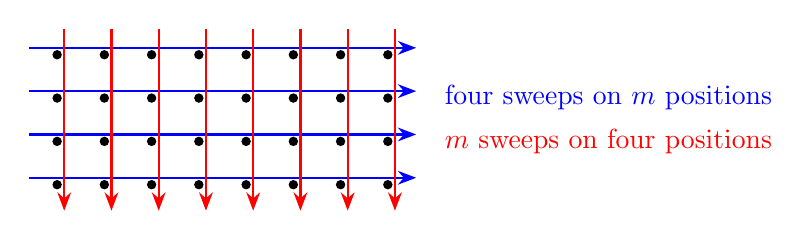
\begin{tikzpicture}[x=0.60cm,y=0.55cm,>=Stealth]
\foreach \i in {0,...,3}{\foreach \j in {0,...,7}{\fill (\j,-\i) circle (1.7pt);}}
\foreach \i in {0,...,3}{\draw[->,blue,thick] (-.6,-\i+.16)--(7.6,-\i+.16);}
\foreach \j in {0,...,7}{\draw[->,red,thick] (\j+.15,.6)--(\j+.15,-3.6);}
\node[blue,anchor=west] at (8,-1) {four sweeps on $m$ positions};
\node[red,anchor=west] at (8,-2) {$m$ sweeps on four positions};
\end{tikzpicture}
\caption{The four rows are indexed by the last two processed bits. The horizontal sweeps occur first; the vertical two-axis sweeps occur last. The number of columns shown is schematic.}\label{fig:fourrows}
\end{figure}

\paragraph{A positive trace for each row type.}
Fix an even integer $r\ge2$, and put
\[
 F_r(\lambda)=D_\lambda\Tr B_{|\lambda|}(\lambda)^r.
\]
We suppress the subscript $r$ while deriving the recursion. Set $X=A^{r/2}$ and $Y=(M^*M)^{r/2}$. The Araki--Lieb--Thirring inequality for positive operators, with exponent $r/2\ge1$ and outer power two, gives
\begin{equation}\label{eq:alt}
 F(\lambda)\le D_\lambda\Tr(XYXY)_\lambda
 =D_\lambda\|Y^{1/2}X_\lambda Y^{1/2}\|_{\HS}^2.
\end{equation}
Indeed $MAM^*$ and $A^{1/2}M^*MA^{1/2}$ have the same nonzero eigenvalues, after which the stated positive-matrix inequality applies \cite{araki1990}; see also the formulation in \cite[Theorem~1]{audenaert2007}.

The row operator $X=A^{r/2}$ is a positive element of the group algebra of
$H$. Let $\mathcal I(\lambda)$ be the set of tuples
$\boldsymbol\alpha=(\alpha_1,\ldots,\alpha_4)$, $\alpha_i\vdash m$,
occurring in $\Res_H V_\lambda$. For each tuple let
$X_{\boldsymbol\alpha}$ be $X$ multiplied by its central isotype
projection in the group algebra of $H$. This projection commutes with $X$,
so the summand is positive in every unitary representation. On $V_\lambda$
it acts on all copies of that row type, not on a chosen copy.
The Hilbert--Schmidt triangle inequality in \eqref{eq:alt} gives
\begin{equation}\label{eq:triangle}
 F(\lambda)^{1/2}\le
 \sum_{\boldsymbol\alpha\in\mathcal I(\lambda)}
 \bigl(D_\lambda\Tr(X_{\boldsymbol\alpha}Y
                         X_{\boldsymbol\alpha}Y)_\lambda\bigr)^{1/2}.
\end{equation}
We now estimate one term of this sum. In every irreducible representation,
$\Tr(X_{\boldsymbol\alpha}Y X_{\boldsymbol\alpha}Y)$ is the squared
Hilbert--Schmidt norm of $Y^{1/2}X_{\boldsymbol\alpha}Y^{1/2}$ and is
nonnegative. The regular representation of $S_N$ contains $D_\lambda$
copies of $V_\lambda$. Its trace therefore bounds the quantity inside
the corresponding square root in \eqref{eq:triangle}. Working in this
larger representation will allow us to express the bound as a probability.

\paragraph{From coefficients to an overlap probability.}
Fix the tuple $\boldsymbol\alpha$. Write
$X_{\boldsymbol\alpha}=\sum_{p\in H}\xi(p)p$, where
$\xi(p)=\prod_i\xi_i(p_i)$. Each row factor has Fourier block
$B_m(\alpha_i)^{r/2}$ on $\alpha_i$ and zero blocks elsewhere.
Plancherel on $S_m$ gives
\[
 m!\sum_{p_i}|\xi_i(p_i)|^2
 =D_{\alpha_i}\Tr B_m(\alpha_i)^r=F(\alpha_i).
\]
If one of these quantities is zero, the tuple contributes nothing.
Otherwise the squared coefficients define probability laws
$u_i(p_i)=|\xi_i(p_i)|^2/\sum|\xi_i|^2$ on the four row groups.
Write $u=\bigotimes_i u_i$ for their independent product.

Because $r/2$ is an integer, $Y=(M^*M)^{r/2}$ is convolution by a
probability law $\omega$ on the column group. Expanding the regular trace gives
\[
 N!\sum_{p,q\in H}\sum_{b,c}\xi(p)\xi(q)\omega(b)\omega(c)
                       \one_{\{p b q c=e\}}.
\]
Bound each coefficient product by
$|\xi(p)\xi(q)|\le(|\xi(p)|^2+|\xi(q)|^2)/2$.
The two square terms have equal sums: cyclically interchange $(p,b)$
and $(q,c)$ in the identity $pbqc=e$. For fixed $p,b,c$, there is
at most one possible $q$, and it lies in $H$ exactly when
$b^{-1}p^{-1}c^{-1}\in H$.
Self-adjointness gives $\xi(p^{-1})=\overline{\xi(p)}$, so $u$ is
invariant under inversion; the real probability coefficients of the
self-adjoint $Y$ have the same symmetry. We may thus invert each of
the three independent variables. Using the preceding Plancherel
normalizations yields
\begin{equation}\label{eq:coefficient-trace}
 \Tr_{\rm reg}(X_{\boldsymbol\alpha}Y
                         X_{\boldsymbol\alpha}Y)
 \le\prod_i F(\alpha_i)\,
 \frac{N!}{(m!)^4}\Pp\{bpc\in H\},
\end{equation}
where $p\sim u$, and $b,c$ are independent column permutations of law
$\omega$. The remaining problem is to bound this overlap probability
uniformly in the squared-coefficient laws $u_i$.

\paragraph{Two independent colorings.}
Let $a(z)$ be the row index of position $z$, and define
\[
 \eta(z)=a(c^{-1}z),\qquad \zeta(z)=a(bz).
\]
The condition $bpc\in H$ is equivalent to
$\zeta(pz)=\eta(z)$ for every position $z$: substitute $z=cw$ in
$a(bpcw)=a(w)$. In each column, either coloring uses the four colors
once. Different columns are independent, and the two colorings are
independent because $b$ and $c$ are.

For row $i$, define a transition matrix on all $4^m$ color strings by
\[
 U_i(x,y)=\Pp_{p_i\sim u_i}\{y(p_i z)=x(z)\text{ for every position }z
                         \text{ in row }i\}.
\]
Thus $U_i$ averages the permutation action of the row group on strings.
Conditional on the two colorings, the four row permutations are
independent. With $\eta_i,\zeta_i$ denoting their restrictions to row $i$,
\[
 \Pp\{bpc\in H\}=\E\prod_i U_i(\eta_i,\zeta_i).
\]
The matrices $U_i$ are stochastic and symmetric, since each $u_i$ is
invariant under inversion. The particular origin of $u_i$ gives the
additional positivity needed in \eqref{eq:interpolation}. Fourier
inversion writes
$\xi_i(g)=(D_{\alpha_i}/m!)\Tr(Q\rho_{\alpha_i}(g^{-1}))$ with
$Q=B_m(\alpha_i)^{r/2}\ge0$. Hence $\xi_i$, and then
$|\xi_i|^2$, are positive-definite functions. Their Fourier transforms
are positive semidefinite, so the average of $u_i$ in the color-string
representation is positive semidefinite as well.

The four-site law of $M$ sends every site exactly uniformly to the four sites. Its adjoint does too, and the same remains true of every positive power of $M^*M$. Moreover the support of $M^*M$ contains the identity and the edge transpositions of the square, which generate $S_4$. Its convolution powers therefore converge to uniform. Choose the even integer $r$ sufficiently large that the law of each column of $Y$ satisfies Theorem~\ref{thm:permanent}. Every larger even $r$ does too, once a tail threshold for convergence has been chosen.

\paragraph{Closing the recursion.}
The variables defining $(\eta_i,\zeta_i)$ consist of $2m$ independent
four-color column assignments. Apply Lemma~\ref{lem:tensorization} to
these assignments with the four nonnegative functions $U_i$, and then
\eqref{eq:interpolation} with $s=4^m$. This gives
\[
 \Pp\{bpc\in H\}
 \le\prod_i\left(s^{-2}\sum_{x,y}U_i(x,y)^{p_0}\right)^{1/p_0}
 \le s^{-4}\prod_i(\Tr U_i)^\theta,
 \quad\theta=1-1/p_0<\frac12.
\]
Since $N!/(m!)^4\le4^N=s^4$, the exponential factors cancel exactly. The only remaining inflation is a power of the four color-string traces. Write $c^\alpha_{\boldsymbol\beta}$ for the multiplicity of $\bigotimes_{i=1}^4V_{\beta_i}$ in the restriction of $V_\alpha$ to $\prod_{i=1}^4S_{|\beta_i|}$. Section~\ref{sec:multiplicities} proves
\begin{equation}\label{eq:trace-C}
 \Tr U_i\le C(\alpha_i),\qquad
 C(\alpha)=\sum_{\boldsymbol\beta}(c^{\alpha}_{\boldsymbol\beta})^2.
\end{equation}
The sum includes every weak four-part composition of $m$ and every
irreducible tuple for its Young subgroup. Combining this trace bound
with \eqref{eq:coefficient-trace} and \eqref{eq:triangle} gives
\begin{equation}\label{eq:recursion}
 F(\lambda)^{1/2}\le
 \sum_{\boldsymbol\alpha\in\mathcal I(\lambda)}
       \prod_{i=1}^4\left(F(\alpha_i)C(\alpha_i)^\theta\right)^{1/2}.
\end{equation}
All restriction multiplicities have been retained; they are accounted for by the regular trace and by $C(\alpha)$, rather than discarded during a choice of one copy.

\section{Squared multiplicities and hook deficits}\label{sec:multiplicities}
We write $\chi_\alpha$ for the character of $V_\alpha$ and
$\langle f,g\rangle_{S_m}=(m!)^{-1}\sum_{x\in S_m}f(x)\overline{g(x)}$ for the normalized character inner product. The cost $C(\alpha)$ in \eqref{eq:recursion} measures how many copies can occur when colors divide a row into four parts. We first justify this interpretation, then bound the cost by boxes outside a thin hook.

\begin{lemma}[Color-string trace]\label{lem:color-trace}
Let $\alpha\vdash m$, let $Q\ge0$ be a nonzero operator on $V_\alpha$, and define the probability
\[
 u(g)=\frac{D_\alpha}{m!\Tr Q^2}
             |\Tr(Q\rho_\alpha(g))|^2\quad(g\in S_m).
\]
Let $U$ be its average action on strings of length $m$ over four colors. Then
\[
 \Tr U\le\langle\chi_\alpha^2,4^{\#\mathrm{cycles}}\rangle_{S_m}
 =\sum_{\boldsymbol\beta}(c^{\alpha}_{\boldsymbol\beta})^2=C(\alpha).
\]
\end{lemma}
\begin{proof}
Schur orthogonality normalizes $u$ to have mass one. Write
$V_\alpha\otimes\overline{V_\alpha}=\bigoplus_\nu V_\nu\otimes\mathbb C^{a_\nu}$, and let $P_\nu$ be its isotypic projection. Character orthogonality gives
\[
 \sum_g u(g)\chi_\nu(g)
 =\frac{D_\alpha\Tr((Q\otimes\bar Q)P_\nu)}
               {D_\nu\Tr Q^2}.
\]
The two commuting positive operators $Q\otimes I$ and $I\otimes\bar Q$ satisfy
\[
 Q\otimes\bar Q\le\tfrac12(Q^2\otimes I+I\otimes\bar Q^2).
\]
The partial trace of $P_\nu$ over either factor commutes with the irreducible action on the other. Its trace is $a_\nu D_\nu$, so it equals
$(a_\nu D_\nu/D_\alpha)I$. The preceding character average is therefore at most $a_\nu$.

A permutation fixes exactly $4^{\#\mathrm{cycles}(g)}$ color strings. This is a permutation character, so its expansion in irreducible characters has nonnegative integer coefficients. Apply the preceding inequality to that expansion. It yields the first asserted bound, since $a_\nu$ is the multiplicity of $\nu$ in $\chi_\alpha^2$.

Finally the color-string representation is the direct sum, over all color-class sizes $m_1+\cdots+m_4=m$, of
$\Ind_{S_{m_1}\times\cdots\times S_{m_4}}^{S_m}\one$.
Frobenius reciprocity identifies its inner product with $\chi_\alpha^2$ as the sum of the dimensions of the commuting algebras of the corresponding restrictions of $V_\alpha$. Those dimensions are the sums of squared multiplicities displayed in the statement.
\end{proof}

For a partition $\alpha\vdash m$, put
\[
 k(\alpha)=m-\max(\alpha_1,\alpha'_1),\qquad
 t_h(\alpha)=|\{(i,j)\in\alpha:i>h,\ j>h\}|\quad(h\ge1).
\]
The latter is the number of boxes outside the union of the first $h$ rows and first $h$ columns.

\begin{lemma}[The cost of restriction]\label{lem:restriction-cost}
There is an absolute $C$ such that, for every $\alpha\vdash m$ and integer $h\ge1$,
\begin{equation}\label{eq:restriction-cost}
 \log C(\alpha)\le t_h(\alpha)\log4
       +C(1+h)(1+\sqrt{k(\alpha)})\log(2m).
\end{equation}
\end{lemma}
\begin{proof}
The central estimate for a residual shape $\delta\vdash t$ is
\begin{equation}\label{eq:squared-lr}
 (c^{\delta}_{\gamma_1,\ldots,\gamma_4})^2
 \le\binom{t}{|\gamma_1|,\ldots,|\gamma_4|}\le4^t.
\end{equation}
To prove it, let the multiplicity on the left before squaring be $c$. Restriction and induction dimensions give, respectively,
\[
 c\prod_iD_{\gamma_i}\le D_\delta,
 \qquad
 cD_\delta\le
 \binom{t}{|\gamma_1|,\ldots,|\gamma_4|}\prod_iD_{\gamma_i}.
\]
Multiplying and cancelling the positive dimensions proves \eqref{eq:squared-lr}. It is essential here to combine one restriction estimate and one induction estimate.

Both $C(\alpha)$ and $t_h(\alpha)$ are invariant under conjugation, so orient $\alpha$ with its first row of length $m-k$, where $k=k(\alpha)$. Remove its first $h$ rows and then the first $h$ columns of the remainder. The residual straight diagram $\delta$ has size $t=t_h(\alpha)$. Deleting a first row leaves an interlacing partition, so reversing that deletion adds a horizontal strip. Deleting a first column gives the vertical analogue.

More explicitly, let $\ell\le2h$ be the number of nonempty removed
lines, let their lengths be $a_1,\ldots,a_\ell$, and let $\xi_j$ be
the trivial character of $S_{a_j}$ for a removed row and the sign
character for a removed column. Then
\[
 W=\Ind_{S_t\times S_{a_1}\times\cdots\times S_{a_\ell}}^{S_m}
       (V_\delta\otimes\xi_1\otimes\cdots\otimes\xi_\ell)
\]
contains $V_\alpha$ by the Pieri rules. Thus each multiplicity in a restriction of
$V_\alpha$ is bounded by the corresponding multiplicity in $W$.
We will use this comparison only for tuples $\boldsymbol\beta$
that occur in the original restriction of $V_\alpha$. For those
tuples, the first-row inequality in the Littlewood--Richardson rule says
$\alpha_1\le\sum_i\beta_{i,1}$, and hence
\begin{equation}\label{eq:tail-budget}
 \sum_i(|\beta_i|-\beta_{i,1})\le k.
\end{equation}
Every intermediate diagram in a Pieri chain ending at such a $\beta_i$ is contained in it, and has at most $k$ boxes below its first row. The number of partitions of any size at most $m$ satisfying that condition is at most
\[
 Q_m(k)=(m+1)^{1+2\lceil\sqrt{k}\rceil}.
\]
One way to see this is to choose the first-row length, and encode the tail by its row lengths and column lengths along a Durfee square of side at most $\sqrt k$. Padding the two lists to length $\lceil\sqrt k\rceil$ gives the displayed upper bound. For $k=0$, only the first-row length is needed.

Fix such a final tuple $\boldsymbol\beta$, and put
$H_{\boldsymbol\beta}=\prod_{i=1}^4S_{|\beta_i|}$.
Mackey's formula for $\Res_{H_{\boldsymbol\beta}}W$ indexes the decomposition by
allocations of the residual factor and the $\ell$ strip factors
among these classes. There are at most $(m+1)^{4(\ell+1)}$
allocation matrices. For each allocation, restrict $V_\delta$ to
the four allocated subsets, then add the allocated horizontal or
vertical strips within each color class by Pieri. A chain ending
at $\beta_i$ consists of diagrams contained in $\beta_i$, so every
one obeys the small-tail bound just counted. Choosing the residual
tuple and all subsequent diagrams costs at most
$Q_m(k)^{4(\ell+1)}$. Each Pieri transition is multiplicity free,
and \eqref{eq:squared-lr} bounds the residual multiplicity by
$4^{t/2}$. Therefore
\[
 c^\alpha_{\boldsymbol\beta}
 \le \operatorname{mult}_{\boldsymbol\beta}(\Res_{H_{\boldsymbol\beta}}W)
 \le (m+1)^{4(\ell+1)}Q_m(k)^{4(\ell+1)}4^{t/2}.
\]
There are at most $Q_m(k)^4$ possible final occurring tuples.
Squaring this bound and summing over them gives $4^t$ times
$\exp\{C(1+h)(1+\sqrt k)\log(2m)\}$, proving
\eqref{eq:restriction-cost}. No tail estimate for the other
constituents of $W$ is required.
\end{proof}

The next fact lets us add hook costs along an entire level of the recursion.

\begin{lemma}[Hook deficits under restriction]\label{lem:hook-deficit}
If $c^{\lambda}_{\alpha_1,\ldots,\alpha_4}>0$, then for every integer $h\ge1$,
\begin{equation}\label{eq:hook-deficit}
 \sum_i t_h(\alpha_i)\le t_h(\lambda),
 \qquad \sum_i k(\alpha_i)\le k(\lambda).
\end{equation}
\end{lemma}
\begin{proof}
For the assertion about $k$, orient the parent with its longest side as first row. The first-row inequality gives a bound by its row deficit on the sum of the child row deficits; each child's $k$ is no larger than its row deficit. If the parent's longest side is a column, transpose every partition, which preserves Littlewood--Richardson multiplicities.

Write $s_\nu$ for the ordinary Schur function, and $s_\nu(X\mid Y)$ for its hook-Schur specialization \cite[Definition~1(a)]{orellana-zabrocki2000}. For the assertion about $t_h$, take $h$ ordinary variables $X$, $h$ transpose variables $Y$, and an unlimited ordinary alphabet $Z$. Variables in $X,Y$ have degree zero and those in $Z$ have degree one. The positive hook-Schur tableau rule uses ordinary entries weakly along rows and strictly down columns, and transpose entries strictly along rows and weakly down columns \cite[Section~2]{mason-niese2016}. For $s_\nu(X\mid Y)$, order all $X$ letters before all $Y$ letters, so the ordinary entries occupy a subdiagram. The rule gives
$s_\nu(X\mid Y)\ne0$ exactly when $\nu_{h+1}\le h$.
For completeness, a tableau over $h$ ordinary and $h$ transpose letters cannot fill an $(h+1)$-by-$(h+1)$ square: the ordinary subdiagram has at most $h$ rows, and the transpose-filled remainder has at most $h$ columns in each remaining row. Conversely, fill the first $h$ rows with their ordinary row letters and the remaining boxes with their transpose column letters. This realizes every diagram in that hook.

Writing $p_j$ for the $j$th power sum, the supersymmetric substitution is
\[
 p_j\longmapsto p_j(X)+(-1)^{j-1}p_j(Y).
\]
Applied to the ordinary Schur coproduct, it gives
\[
 s_\lambda(X+Z\mid Y)
 =\sum_{\nu\subseteq\lambda}s_\nu(X\mid Y)s_{\lambda/\nu}(Z).
\]
Its coefficients are nonnegative. The largest subdiagram of $\lambda$ in the $(h,h)$ hook is the union of its first $h$ rows and first $h$ columns. The smallest degree in $Z$ is therefore exactly $t_h(\lambda)$; the corresponding skew Schur function is nonzero on an unlimited alphabet.

Apply this substitution to
$\prod_i s_{\alpha_i}=\sum_\lambda c^{\lambda}_{\boldsymbol\alpha}s_\lambda$.
The product on the left has minimum $Z$-degree $\sum_i t_h(\alpha_i)$. Every summand on the right has nonnegative coefficients, so an occurring parent's minimum degree cannot be smaller. This is \eqref{eq:hook-deficit}.
\end{proof}

Equations~\eqref{eq:recursion} and \eqref{eq:restriction-cost} now give a recursive estimate in which the leading charge is $\theta\log4$ times a hook deficit. The other charges involve only $(1+h)(1+\sqrt k)\log(2m)$. We next prove where this recursion can stop, before summing those charges.

\section{Sparse stopping by encounter forests}\label{sec:sparse}
The four-row recursion will stop when a diagram is close to one row or column. We prove the needed bound directly from the paths of a small collection of cards. Branching expresses the trace for $s$ tracked cards as a binomial sum over first-row deficits. Inverting that sum cancels contributions supported on fewer than all the tracked cards. To preserve this cancellation, we couple all subsets of the tracked cards in one sweep.

Throughout this section, $n=2^d$, $T=T_n$, $B=TT^*$, and $B_\lambda=B_n(\lambda)$. Empty diagrams have dimension one.

\begin{lemma}[Sparse stopping]
\label{lem:sparse}
There is an absolute $N_0$ such that, if $n=2^d\ge N_0$ and
$1\le k\le n^{1/100}$, then
\[
 \sum_{\mu\vdash k}D_\mu\,
     \Tr B_{(n-k,\mu)}\le n^{-3k/10}.
\]
Consequently, for $n\ge N_0$, if
$k(\lambda)=n-\max\{\lambda_1,\lambda'_1\}\le n^{1/100}$,
then for every integer $r\ge4$,
\[
 D_\lambda\Tr B_\lambda^r\le1.
\]
There is a fixed even $r_0\ge4$ for which the latter assertion holds
for every power of two $n\ge2$ and every such $\lambda$.
\end{lemma}

\begin{proof}
\emph{Isolating the first-row deficit.}
Let $\mathcal I_s$ be the set of ordered injections from $[s]$ into
the $n$ positions, with $\mathcal I_0$ a singleton. The sweep induces
a transition matrix $T_s$ on this set. Write
\[
 a_s=\Tr_{\mathbb C^{\mathcal I_s}}(TT^*)
     =\sum_{x,y\in\mathcal I_s}T_s(x,y)^2.
\]
This is the ordinary, unnormalized trace on the indicated permutation module.

The permutation module on $\mathcal I_s$ is
$\operatorname{Ind}_{S_{n-s}}^{S_n}\mathbf1$. By repeated branching,
the multiplicity of $V_\lambda$ in it is the number of standard
tableaux of skew shape $\lambda/(n-s)$. Assume $s\le k$ and
$n\ge2k$. Every occurring partition has the form
$\lambda=(n-j,\mu)$ with $0\le j\le s$ and $\mu\vdash j$.
The skew shape consists of the tail $\mu$ and a row of $s-j$ cells
whose columns exceed $n-s\ge k\ge\mu_1$. These components share
neither a row nor a column. Choosing the $j$ entries of the tail and
then a standard tableau on it gives multiplicity
$\binom{s}{j}D_\mu$. Hence
\[
 a_s=\sum_{j=0}^s\binom{s}{j}b_j,
 \qquad
 b_j=\sum_{\mu\vdash j}D_\mu\,
                \Tr B_{(n-j,\mu)}.
\]
Binomial inversion gives
\begin{equation}
\label{eq:sparse-inverse}
 b_k=\sum_{s=0}^k(-1)^{k-s}\binom{k}{s}a_s\ge0,
\end{equation}
where positivity follows from the positive semidefiniteness of each
$B_\lambda$. It remains to bound this inverse without losing its
cancellation.

For fixed initial and final positions of one card, there is exactly
one possible path through the successive coordinate layers: at layer
$i$, its first $i$ processed coordinates have their final values and
its remaining coordinates still have their initial values. Thus fixed
endpoints for $s$ cards prescribe all their paths. If two tracked cards
use the same switch, the two prescribed coin requirements either
disagree, making the endpoints impossible, or agree, saving one coin.
If $e$ is the number of switches shared by two tracked cards along a
realized sweep, the transition probability to its realized endpoint is
therefore $2^{-ds+e}=n^{-s}2^e$. Averaging first over the realized
endpoint and then over a uniform initial injection gives the exact
identity
\begin{equation}
\label{eq:sparse-trace}
 a_s=\frac{(n)_s}{n^s}\,\mathbb E\,2^e,
 \qquad (n)_s=n(n-1)\cdots(n-s+1).
\end{equation}

Choose $k$ distinct uniform initial positions $X_1,\ldots,X_k$,
independently of the coins of one complete sweep. For this realized
sweep, form a graph $G$ on all $n$ initial positions, joining two
positions if their cards share a switch. Each vertex has degree $d$.
The graph is simple: after two cards meet at coordinate $i$, their
positions differ at that coordinate forever, so they cannot meet at a
later coordinate. Let $G_X$ be the graph induced on the selected tags,
and let $e(S)$ count its edges with both endpoints in $S\subseteq[k]$.
The marginal initial positions of every such subset are a uniform
injection. Thus, with
\[
 w(S)=\frac{(n)_{|S|}}{n^{|S|}}
     =\prod_{i\in S}\left(1-
             \frac{\#\{j\in S:j<i\}}n\right),
\]
Equations~\eqref{eq:sparse-trace} and \eqref{eq:sparse-inverse} imply
\begin{equation}
\label{eq:sparse-coupled}
 b_k=\mathbb E\sum_{S\subseteq[k]}
             (-1)^{k-|S|}w(S)2^{e(S)}.
\end{equation}

A predecessor selection is a collection $D$ of directed pairs
$(i,j)$ with $1\le j<i\le k$, at most one pair having any given
first coordinate. Write $|D|$ for its number of pairs and
$\operatorname{supp}D$ for their endpoints. Expanding the product
defining $w(S)$ gives
\[
 w(S)=\sum_{D:\operatorname{supp}D\subseteq S}
                         (-n^{-1})^{|D|}.
\]
Also $2^{e(S)}=\sum_{H\subseteq E(G_X[S])}1$. If
$\operatorname{supp}H$ denotes the vertices incident to the edges
of $H$, then summing over $S$ in \eqref{eq:sparse-coupled} yields the
exact cancellation identity
\begin{equation}
\label{eq:sparse-cover}
 b_k=\mathbb E\sum_{H\subseteq E(G_X)}\ 
       \sum_{D:\operatorname{supp}H\cup\operatorname{supp}D=[k]}
                     (-n^{-1})^{|D|}.
\end{equation}
Indeed, a term supported on $U$ has coefficient
$\sum_{S\supseteq U}(-1)^{k-|S|}$, which is zero unless $U=[k]$.
Thus only an encounter-edge set and a predecessor selection that
together cover every tag survive the inversion. We may now bound their
absolute sum without losing that covering constraint.

\medskip\noindent
\emph{Counting the covering configurations.}
Two elementary facts about $G$ control the possible encounter
subgraphs. First, every set of $v$ vertices spans at most
\begin{equation}
\label{eq:sparse-edge-count}
 \frac v2\log_2v
\end{equation}
edges, with $0\log_2 0=0$. To prove this by induction on $d$, split
the initial positions according to the last processed coordinate.
Before the last layer, these two halves remain separate. If the
chosen set has $v_0,v_1$ positions in them, induction bounds the
earlier encounters by
$\tfrac12v_0\log_2v_0+\tfrac12v_1\log_2v_1$, and the last matching
adds at most $\min(v_0,v_1)$ edges. This is at most
$\tfrac12v\log_2v$ because the binary entropy
$H_2(p)=-p\log_2p-(1-p)\log_2(1-p)$, with $0\log_2 0=0$, satisfies
$H_2(p)\ge2\min(p,1-p)$ by concavity on each half of $[0,1]$.

Second, if $F$ is a specified forest on $v$ selected tags with $c$
components, then, conditional on the entire sweep,
\begin{equation}
\label{eq:sparse-forest-probability}
 \Pr(F\subseteq G_X\mid G)
 \le\frac{n^cd^{v-c}}{(n)_v}
 \le2\left(\frac dn\right)^{v-c}.
\end{equation}
Choose one root position per component and then successively place
each child at one of at most $d$ neighbors of its parent. This gives
the first inequality even if some counted placements fail to be
injective. For $v\le k\le n^{1/100}$ and sufficiently large $n$,
\[
 \frac{(n)_v}{n^v}
 =\prod_{i=0}^{v-1}(1-i/n)
 \ge1-\frac{v(v-1)}{2n}\ge\frac12,
\]
which gives the second inequality.

Let an encounter-edge set $H$ use $v$ vertices and have $c$ nontrivial
connected components. Then $2c\le v$, and $H$ contains a spanning
forest with $v-c$ edges. For fixed $v,c$, there are at most
$(2k)^{2v}$ choices for its vertex set and forest: choose the vertex
set, root every component at its least vertex, and record a parent
or a root marker for every vertex. For any realization and any such
forest, the number of possible edge sets extending it is at most
\[
 2^{e(G_X[V])}\le v^{v/2}\le k^{v/2},
\]
by \eqref{eq:sparse-edge-count}. A canonical choice of spanning
forest for each $H$, or simply overcounting all spanning forests,
therefore bounds the expected number of these $H$ by
\[
 2(2k)^{2v}k^{v/2}(d/n)^{v-c}.
\]
For $v=c=0$, the empty edge set contributes one, which also obeys
this upper bound.

There are at most $\binom{k}{q}k^q\le(2k)^{2q}$ predecessor
selections with $q$ pairs. The covering condition in
\eqref{eq:sparse-cover} implies $v+2q\ge k$. Since $d/n\le1$,
$v-c\ge v/2$, and there are at most $(k+1)^3$ triples $(v,c,q)$,
the preceding estimates show that
\begin{equation}
\label{eq:sparse-sum}
 b_k\le 2\sum_{\substack{0\le v,c,q\le k\\
                         2c\le v,\ v+2q\ge k}}
       \left(4k^{5/2}\sqrt{d/n}\right)^v
       \left(4k^2/n\right)^q.
\end{equation}
Impossible triples only enlarge this upper bound. Uniformly for
$1\le k\le n^{1/100}$, sufficiently large $n$ satisfies
\[
 4k^{5/2}\sqrt{d/n}\le n^{-2/5},\qquad
 2k/\sqrt n\le n^{-2/5},\qquad
 2(k+1)^3\le n^{k/10}.
\]
For example, the first left side is at most
$4\sqrt{\log_2n}\,n^{-19/40}$, and the last left side is at most
$16n^{3/100}$. Every term in \eqref{eq:sparse-sum} is therefore at
most $n^{-2(v+2q)/5}\le n^{-2k/5}$, proving
$0\le b_k\le n^{-3k/10}$.

\medskip\noindent
\emph{From the trace bound to stopping.}
If $\lambda_1=n-k$ with $1\le k\le n^{1/100}$, its term in $b_k$
has coefficient $D_\mu\ge1$, so
$\Tr B_\lambda\le n^{-3k/10}$. The eigenvalues are
nonnegative, and consequently
\[
 \Tr B_\lambda^r
 \le(\Tr B_\lambda)^r.
\]
Choosing the labels of the $k$ cells below the first row and then
their order gives $D_\lambda\le\binom nk k!\le n^k$. Hence
\[
 D_\lambda\Tr B_\lambda^r
 \le n^{(1-3r/10)k}\le1\qquad(r\ge4).
\]

If instead $\lambda'_1=n-k>n/2$, every matching projection vanishes
on $V_\lambda$. Indeed, its fixed-space dimension is the
multiplicity of $V_\lambda$ in
$\operatorname{Ind}_{S_2^{n/2}}^{S_n}\mathbf1$. Repeated horizontal
Pieri shows that every constituent is obtained by adding $n/2$
horizontal strips of size two. Each strip adds at most one cell to
the first column, so every constituent has first-column height at
most $n/2$. Thus $B_\lambda=0$ in the case under consideration.
For $k=0$, the trivial representation has the claimed value one
and the sign representation is annihilated by a matching projection.

Finally, Lemma~\ref{lem:gap} gives operator norm strictly less than
one on every nontrivial irreducible at each fixed $n$.
There are only finitely many powers of two below $N_0$ and finitely
many irreducibles at each of them. Increasing $r$ to one fixed even
$r_0\ge4$ therefore gives the stated stopping estimate also at these
remaining sizes. Larger powers preserve the estimate because $B$
is a positive semidefinite contraction.
\end{proof}

\section{Summing the costs and comparing dimensions}\label{sec:tree}
We now assemble the recursion. The purpose of the sparse estimate is to prevent costs from accumulating indefinitely on diagrams with a long row or column. The remaining costs can be summed before we compare them with the dimension of the root.

Write $\log^+x=\max\{0,\log x\}$. Fix a root $\lambda\vdash N$, with $K=k(\lambda)>0$. A node with diagram $\alpha\vdash m$ is expanded only if $m$ exceeds a fixed cutoff $M$ and $k(\alpha)>m^{.01}$. Otherwise it is stopped. Choose the even moment $r$ large enough for Lemma~\ref{lem:sparse} and, by Lemma~\ref{lem:gap}, large enough that $F(\alpha)\le1$ for every stopped diagram of size at most $M$. These choices are possible simultaneously. The numerical cutoff will be fixed below before $r$ is finally chosen.

Squaring \eqref{eq:recursion} and bounding a sum by its number of terms times its largest term gives
\begin{equation}\label{eq:log-recursion}
 \log F(\alpha)\le2\log|\mathcal I(\alpha)|
 +\max_{\boldsymbol\beta\in\mathcal I(\alpha)}
     \sum_{i=1}^4\{\log F(\beta_i)+\theta\log C(\beta_i)\}.
\end{equation}
We use $\log0=-\infty$. If $F(\alpha)=0$, no bound is needed. Iterating this inequality amounts to taking the maximum over finite four-ary trees of occurring restrictions. Each expanded node contributes its choice cost $2\log|\mathcal I(\alpha)|$, and each of its four immediate children contributes $\theta\log C(\beta_i)$. The latter charge remains present even if the child is stopped.

The tail count in the proof of Lemma~\ref{lem:restriction-cost} gives
\[
 \log|\mathcal I(\alpha)|
 \le C(1+\sqrt{k(\alpha)})\log(2m).
\]
To apply it, orient the parent along its longest side, use the first-row inequality, and count each child's tail with at most the parent's deficit. Child sizes are prescribed. Thus this choice cost fits within the lower-order term of \eqref{eq:restriction-cost}. We may charge it at the parent, including the root, without altering the estimates below.

For $H>2$, put
\[
 R_H(\lambda)=\sum_{(i,j)\in\lambda}\log^+\frac{\min(i,j)}H.
\]
This quantity will count, box by box, the levels at which a root box
can lie outside the chosen hook. The budget below adds an entropy
term $\tfrac12K\log(N/K)$. Lemma~\ref{lem:hook-comparison} will
compare $R_H(\lambda)+K\log(N/K)$ with $\log D_\lambda$, with
explicit errors. We therefore seek a coefficient below one in front
of the budget, leaving room to absorb its lower-order costs.

\begin{lemma}[Uniform tree budget]\label{lem:tree-budget}
Fix $\delta\in(0,1/2)$ and put $a=1/2-\delta$. For every $H>2$ and $\epsilon>0$, a sufficiently large fixed cutoff $M$ makes every such recursion tree satisfy
\begin{equation}\label{eq:tree-budget}
 \log F(\lambda)\le\epsilon K+
 \frac\theta a\left\{
    R_H(\lambda)+\frac K2\log\frac NK\right\}.
\end{equation}
The cutoff and all constants in this statement are independent of the final even moment $r$.
\end{lemma}
\begin{proof}
At a level with node size $m$, let $q_m$ be the number of charged nodes and let their deficits be $k_1,\ldots,k_{q_m}$. By Lemma~\ref{lem:hook-deficit}, their sum is at most $K$. Expanded nodes satisfy $k_i>m^{.01}$, so their number is at most $K/m^{.01}$. A charged child of size $m$ has an expanded parent of size $4m$, and there are four children per parent. Consequently, after changing one absolute constant,
\begin{equation}\label{eq:charged-count}
 q_m\le C K m^{-.01},\qquad q_m\le N/m,
 \qquad\sum_i k_i\le K.
\end{equation}
The root also satisfies these bounds when expanded. A stopped root already has $F\le1$ and satisfies the conclusion directly.

At that level choose
\[
 h_m=\left\lceil m^a\sqrt{K/N}\right\rceil.
\]
The lower-order terms in the choice and restriction costs are bounded by
\[
 C\sum_i(1+h_m)(1+\sqrt{k_i})\log(2m).
\]
Cauchy--Schwarz gives $\sum_i\sqrt{k_i}\le\sqrt{q_mK}$. The terms arising from the ceiling and the constant one are therefore at most
$CKm^{-.005}\log(2m)$. For the terms involving $m^a$, use both bounds in \eqref{eq:charged-count}:
\[
 m^a\sqrt{K/N}\sqrt{q_mK}\le Km^{-\delta},
\]
\[
 m^a\sqrt{K/N}\,q_m
 \le CKm^{-\delta-.005}.
\]
For the second inequality, $q_m\le\sqrt{(N/m)(CK/m^{.01})}$. These costs are summable geometric tails because level sizes differ by a factor four. All charged nodes have size greater than $M/4$, including the stopped children of the last expanded level. Choosing $M$ large makes their total at most $\epsilon K$.

It remains to sum the leading hook terms. At every level, iteration of Lemma~\ref{lem:hook-deficit} bounds the sum of $t_{h_m}$ over charged nodes by $t_{h_m}(\lambda)$. Follow one root box $(i,j)$ and write $s=\min(i,j)$. It can contribute only if
\[
 s>h_m\ge m^a\sqrt{K/N}.
\]
The eligible sizes $m$ form part of a geometric progression of ratio four, all larger than $M/4$. By increasing $M$ so that $(M/4)^a\ge4^a H$, their number is at most
\[
 \frac{\log^+(s/H)+\tfrac12\log(N/K)}{a\log4}.
\]
Indeed the number is bounded by the positive part of one plus the logarithm of the ratio of the upper endpoint
$(s\sqrt{N/K})^{1/a}$ to the lower endpoint $M/4$, divided by $\log4$; the choice of $M$ absorbs the extra one. Replacing $\log(s/H)$ by its positive part can only enlarge the bound.

Boxes in the longest first row or column never contribute, since $h_m\ge1$. There are exactly $K$ remaining boxes. Multiply their level counts by $\theta\log4$ and add the lower-order costs. This proves \eqref{eq:tree-budget}.
\end{proof}

We have reduced the operator recursion to a purely diagrammatic comparison. The next lemma compares $R_H(\lambda)$ with the hook-length formula, retaining the first-row entropy needed when $K$ is small relative to $N$.

\begin{lemma}[Hook comparison]\label{lem:hook-comparison}
Orient $\lambda\vdash N$ so its first row is a longest side, put $K=N-\lambda_1>0$, and let $\zeta=(\lambda_2,\lambda_3,\ldots)\vdash K$. For $H>2$,
\begin{align}
 \log D_\lambda
 &\ge K\log(N/K)+\log D_\zeta-E_{N,K},\label{eq:row-hook}\\
 R_H(\lambda)&\le\log D_\zeta+4K/H,\label{eq:rank-hook}
\end{align}
where $E_{N,K}=O(K/N)$ for $K<N/3$ and
$E_{N,K}=O(\sqrt N\log(2N))$ for $K\ge N/3$.
There is also an absolute $c>0$ such that
$\log D_\lambda\ge cK$ for all sufficiently large $N$ and every nontrivial, nonsign $\lambda$.
\end{lemma}
\begin{proof}
The hook-length formula separates the first row exactly:
\[
 D_\lambda=\binom NKD_\zeta
 \prod_{j=1}^{\lambda_1}
 \left(1+\frac{\lambda'_j-1}{\lambda_1-j+1}\right)^{-1}.
\]
If $K<N/3$, a nonzero numerator occurs only for $j\le K$, so the logarithm of the inverted product is at most $K/(N-2K+1)$. For $K\ge N/3$, split the columns at height $\sqrt N$. There are at most $\sqrt N$ columns taller than this; each contributes at most $\log(1+N)$. In the remaining columns, bound $\log(1+x)$ by $x$ and sum the denominators harmonically. Their contribution is at most $\sqrt N(1+\log N)$. Since $\binom NK\ge(N/K)^K$, this proves \eqref{eq:row-hook}.

Every box contributing to $R_H$ lies in $\zeta$. At root coordinates $(i,j)$, its hook in $\zeta$ has length at most
\[
 \frac K{i-1}+\frac Kj\le\frac{4K}{\min(i,j)}.
\]
Take a reverse linear extension of the Young diagram order on $\zeta$, numbering its boxes from $1$ to $K$. The number assigned to each box is at least its hook length, because all boxes to its right and below precede it. The product of all number-to-hook ratios is exactly $D_\zeta$, and every ratio is at least one.

Suppose $t$ boxes contribute to $R_H$. Their distinct assigned numbers have product at least $t!$. Keeping only their ratios in the hook product gives, for $t>0$,
\[
 \log D_\zeta\ge R_H-t\log\frac{4eK}{tH}
 \ge R_H-\frac{4K}H.
\]
The last inequality follows by maximizing $t\log(4eK/(tH))$ over $t>0$. For $t=0$, the assertion is immediate.

Finally we prove $\log D_\lambda\ge cK$ without losing uniformity in the shape. If $K<N/3$, \eqref{eq:row-hook} already gives this for large $N$. Put $L=\lambda_1=\max(\lambda_1,\lambda'_1)$. If $K\ge N/3$ and $L\ge N/8$, retain the first row and an order ideal of $b=\lfloor N/32\rfloor$ boxes in the lower diagram. Place $1,\ldots,b$ in the first $b$ boxes of the top row, choose any $b$ of the remaining $L$ labels for the lower diagram, fill those lower boxes in a fixed standard order, and fill the rest of the top row increasingly. This gives $\binom Lb\ge4^b$ standard tableaux of the retained diagram. Every such tableau extends to $\lambda$. If $L<N/8$, every hook is shorter than $N/4$, so
$D_\lambda\ge N!/(N/4)^N\ge(4/e)^N$.
These cases give one absolute positive $c$.
\end{proof}

\begin{proof}[Proof of the moment assertion in Theorem~\ref{thm:moment}]
Fix the constants in their logical order. Theorem~\ref{thm:permanent} first gives $p_0$ and $\theta<1/2$. Choose $\delta>0$ so small that
\[
 b:=\frac\theta{1/2-\delta}<1.
\]
The universal degree constant $c$ in Lemma~\ref{lem:hook-comparison} is independent of this choice. Choose $H$ sufficiently large and $\epsilon$ sufficiently small that
$\epsilon+4b/H<(1-b)c/4$. Then choose the cutoff $M$ required by Lemma~\ref{lem:tree-budget}, increasing it further so that the errors $E_{N,K}$ in Lemma~\ref{lem:hook-comparison} are less than $(1-b)cK/(4b)$ whenever $N>M$. This is possible uniformly: the first error divided by $K$ is $O(1/N)$, and the second is $O(\log N/\sqrt N)$ in its stated range.

Only now choose the even moment $r$. It must make the four-site column law admissible for Theorem~\ref{thm:permanent}, enforce the sparse stopping rule, and make $F_r\le1$ for all nontrivial shapes of all dyadic sizes at most $M$. These are finitely many or fixed-threshold requirements, by Lemmas~\ref{lem:gap} and \ref{lem:sparse}; all persist on increasing $r$.

For an expanded root, \eqref{eq:tree-budget}, \eqref{eq:row-hook} and \eqref{eq:rank-hook} give
\[
 \log F_r(\lambda)
 \le b\log D_\lambda+\epsilon K+4bK/H+bE_{N,K}
 \le\frac{1+b}{2}\log D_\lambda.
\]
Here we discarded the additional negative term
$-bK\log(N/K)/2$. Thus $\eta=(1-b)/2>0$ works at every expanded root. At a stopped root $F_r\le1\le D_\lambda^{1-\eta}$. The row representation has $F_r=1$, while the column representation is killed by Lemma~\ref{lem:gap}. This proves the moment assertion for every dyadic $N$.
\end{proof}

\section{Independent forward sweeps}\label{sec:amplification}
The estimate just proved concerns the positive operator $B_N=T_NT_N^*$. Actual repeated shuffles use powers of $T_N$. We make that distinction explicit in the final argument.

First, the degree estimates above imply, for any fixed $A>0$,
\begin{equation}\label{eq:degree-sum}
 \sum_{\lambda\ne(N),(1^N)}D_\lambda^{-A}\longrightarrow0.
\end{equation}
Here are the elementary summability details. There are at most $2p(k)$ partitions with $k(\lambda)=k$, because deleting the longer first row or column leaves a partition of $k$. The partition generating function gives $p(k)\le e^{3\sqrt k}$: evaluate it at $x=e^{-1/\sqrt k}$, and bound its logarithm by
\[
 \sum_{j\ge1}\frac1{j(e^{j/\sqrt k}-1)}
 \le\sqrt k\sum_{j\ge1}j^{-2}\le2\sqrt k.
\]
Lemma~\ref{lem:hook-comparison} bounds $D_\lambda^{-A}$ by $e^{-Ac k}$ for all sufficiently large $N$. The resulting bound $2e^{3\sqrt k-Ack}$ is summable in $k$. For each fixed $k\ge1$, the first-row hook identity gives $D_\lambda\to\infty$ as $N\to\infty$, uniformly over those finitely many tails. Dominated convergence proves \eqref{eq:degree-sum}. This elementary argument suffices here; more precise fixed-exponent degree sums are known \cite{liebeck-shalev2004}.

From \eqref{eq:moment},
\[
 \|B_N(\lambda)\|_{\op}^r\le\Tr B_N(\lambda)^r
 \le D_\lambda^{-\eta}.
\]
Thus, for any integer $q\ge r$, Schatten H\"older and the operator norm bound give
\[
 \|T_N(\lambda)^q\|_{\HS}^2
 \le\|T_N(\lambda)\|_{\op}^{2(q-r)}
                 \|T_N(\lambda)\|_{2r}^{2r}
 =\|B_N(\lambda)\|_{\op}^{q-r}\Tr B_N(\lambda)^r.
\]
Multiplying by $D_\lambda$ and using the moment theorem yields
\begin{equation}\label{eq:forward-power}
 D_\lambda\|T_N(\lambda)^q\|_{\HS}^2
 \le D_\lambda^{1-\eta q/r}.
\end{equation}
Choose once and for all an integer $q>r/\eta$. Equation~\eqref{eq:degree-sum} shows that the sum of \eqref{eq:forward-power} over all nonsign, nontrivial representations tends to zero. The sign block is zero.

For clarity, finite-group Plancherel and Cauchy--Schwarz state that any probability $\sigma$ on $S_N$ satisfies
\[
 4\|\sigma-U_{S_N}\|_{\TV}^2
 \le N!\sum_g|\sigma(g)-1/N!|^2
 =\sum_{\lambda\ne(N)}D_\lambda
                     \|\widehat\sigma(\lambda)\|_{\HS}^2.
\]
Apply this to $\sigma=\mu_N^{*q}$, whose Fourier matrix is $T_N(\lambda)^q$. This proves convergence to uniform after $q$ forward sweeps. Translating the law by any deterministic starting deck preserves total variation, so the result is uniform over starting states. A sweep is $d$ physical shuffles, giving the asserted $O(d)$ bound. The support estimate \eqref{eq:support-intro} supplies the matching lower order.

No step identifies $(T_NT_N^*)^q$ with $T_N^q(T_N^*)^q$. The positive moment supplies singular-value information; H\"older is the separate passage to forward evolution.

\begingroup\small
\bibliographystyle{plain}
\bibliography{references}
\endgroup
\end{document}
